%Question 3
\def \Cp{1 \; F}
\def \Rp{1 \; \Omega}
\def \C{100 \; nF}
\def \wc{(2\pi \; rad)(1000 \; Hz) }
\def \wcp{1.5538 \; rad/s}
\def \Kf{4043.8220}
\def \Km{2472.9081}
\def \R{2472.9081 \; \Omega}
\def \wh{4.0438 \times 10^3}
\begin{enumerate}
	
	%Part a
	\item{
	
	Filter will have the structure:
	
	INSERT DIAGRAM HERE!
	%INSERT DIAGRAM HERE!	
	
	For the filter stages, will use prototype filters and scaling to find values of components.
	
	\begin{align*}
	&R_p = \Rp
	\\
	&C_p = \Cp
	\end{align*}		
	
	To find prototype cutoff frequency, must solve:
	$$ |H(j\omega_c)| = \frac{1}{\sqrt{2}} H_{max} $$
	
	\begin{align*}
	& \left| \left( \frac{j \omega_c}{j \omega_c + 1} \right)^n \right| = \frac{1}{\sqrt{2}}
	\\
	\implies & \frac{\omega_c^n}{\left( \sqrt{\omega_c^2 + 1} \right)^n} = \frac{1}{\sqrt{2}}
	\\
	\implies & \frac{\omega_c^n}{\left( \omega_c^2 + 1 \right)^{\frac{n}{2}}} = \frac{1}{2^{\frac{1}{2}}}
	\\
	\implies & \frac{\omega_c^{2n}}{\left( \omega_c^2 + 1  \right)^n} = \frac{1}{2}
	\\
	\implies & \omega_c^2 - 2^{\frac{1}{n}}\omega_c^2 + 1 = 0
	\\
	\implies & \omega_c = \pm \frac{1}{\sqrt{\sqrt[n]{2} - 1}}
	\\
	&\omega_c > 0
	\\
	\implies & \omega_c =  \frac{1}{\sqrt{\sqrt[n]{2} - 1}}
	\end{align*}	
	
	Therefore, for our prototype cascaded filter:
	$$ \omega_{cp} = \frac{1}{\sqrt{\sqrt[2]{2}} - 1} = \wcp $$	
	
	Frequency scaling: 
	\begin{align*}
	K_f &= \frac{\omega_c}{\omega_{cp}}
	\\
	&= \frac{\wc}{\wcp}
	\\
	&= \Kf
	\end{align*}
	
	Magnitude scaling:
	\begin{align*}
	C &= \frac{1}{K_f K_m} C_p
	\\
	\implies K_m &= \frac{C_p}{K_f C}
	\\
	&= \frac{\Cp}{(\Kf) (\C)}
	\\
	&= \Km
	\end{align*}
	
	Resistor Value:
	\begin{align*}
	R &= K_m R_p
	\\
	&= (\Km)(\Rp)
	\\
	&= \R
	\end{align*}
	
	Gain stage:\\
	Resistors in the gain stage are independent of the frequency response of the circuit, 
	and are just chosen to get the correct gain. For this configuration of op-amp:
	$$ G = 1 + \frac{R_f}{R_s} $$
	For a gain of $10$, choosing $R_f = 9 \; K\Omega$ gives $R_s = 1 \; K\Omega$. 
	
	INSERT DIAGRAM OF COMPLETED CIRCUIT WITH VALUES HERE:
	%INSERT DIAGRAM HERE!	
	
	}
	
	%Part b
	\item{
	Transfer function of the whole circuit is the product of the transfer function of
	each stage in the amplifier, noting that stage 1 and stage 2 are identical:
	
	$$ H(s) = (H_1(s))^2 H_3(s) $$
	
	Where $H_1(s)$ is the transfer function for one amplification stage and 
	$H_3(s)$ is the transfer function for the gain stage.\\
	As $H_3(s)$ is frequency independent, we can say that $H_3(s) = 10 $\\
	
	For the amplification stage:
	High pass filter has a transfer function in the form 
	$$H(s) = \frac{-R_f}{R_s}\frac{s}{s + \frac{1}{R_sC}}$$
	For our amplification stages, $R_f = R_s = \R$ and $C = \C$.
	Therefore:
	
	\begin{align*}
	H_1(s) &= \frac{- \R}{\R} \frac{s}{s + \frac{1}{(\R)(\C)}}
	\\
	&= \frac{s}{s + \wh }
	\\
	H(s) &= (H_1(s))^2H_3(s)
	\\
	&= 10 \left( \frac{s}{s + \wh } \right)^2 
	\\
	&= \frac{10 s^2}{s^2 + (8.0876\times 10^3) s + 16.3525 \times 10^6}
	\end{align*}
	}
	
	%Part c
	\item{
	\text{}
	\begin{figure}[H]
	\begin{center}
	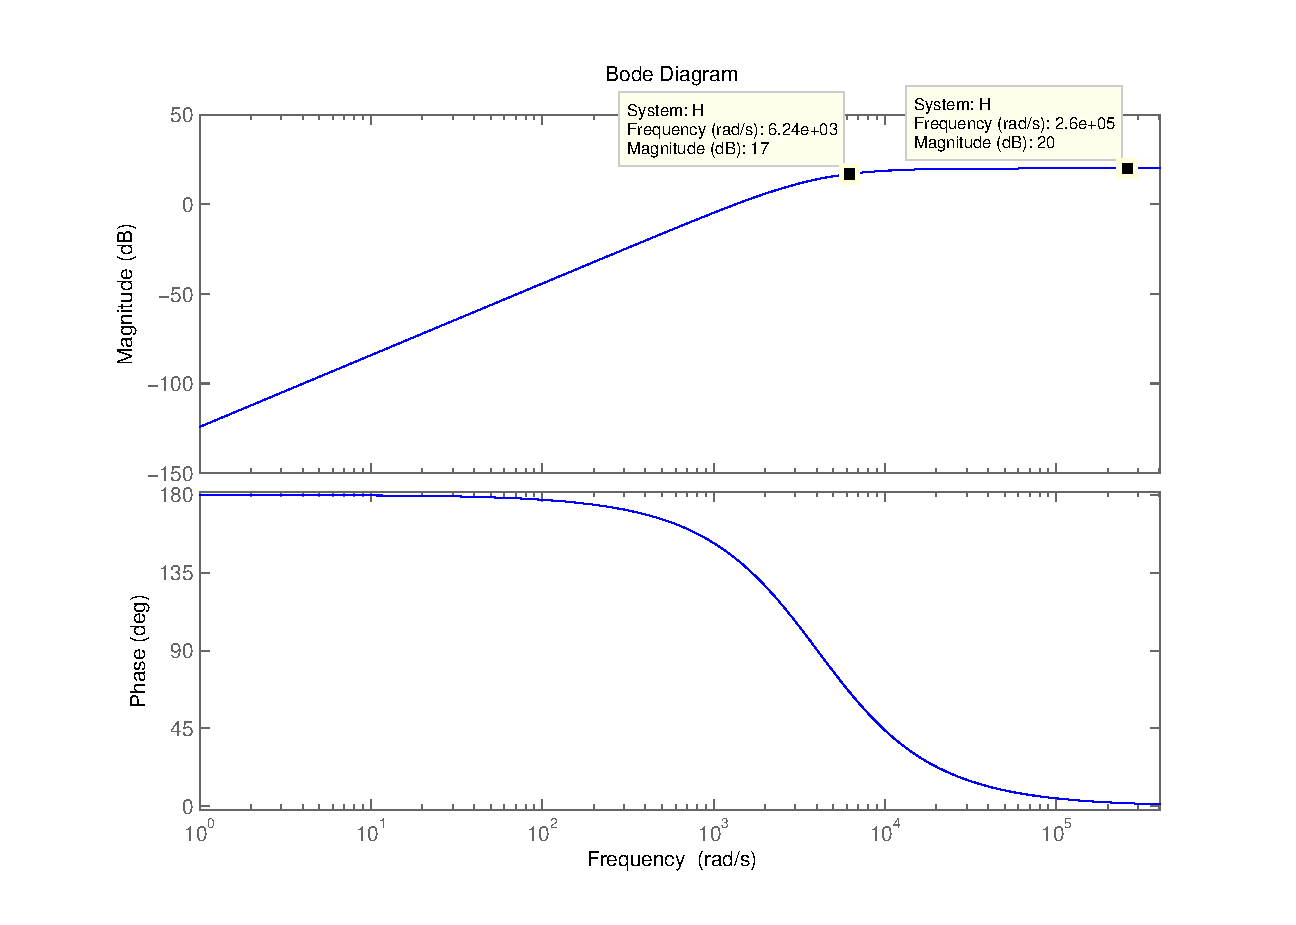
\includegraphics[scale=0.75]{q3bode}
	\end{center}
	\end{figure}
	}
	\begin{align*}
	6.24 \times 10^3 \; rad/s &= \frac{6.24 \times 10^3}{2\pi} \; Hz
	\\
	&= 993.127 \; Hz
	\\
	&\approx 1000 \; Hz
	\end{align*}
	Therefore, this transfer function satisfies the specifications.
	
	
\end{enumerate}